\documentclass[]{scrartcl}
\title{Vorlesung Analysis II}
\usepackage{amsmath,amssymb,amsfonts}
\usepackage{stmaryrd}
\usepackage{mathtools}
\usepackage{latexsym}
\usepackage{graphicx}
\usepackage{tikz}
\usepackage{xcolor}
\usepackage[most]{tcolorbox}
\usepackage{soul}
\usepackage{ upgreek }
\usepackage{hyperref}
\usepackage{tipa}
\usepackage[dvipsnames]{xcolor}
\hypersetup{
	colorlinks=true,
	linkcolor=blue,
	filecolor=magenta,      
	urlcolor=cyan,
	pdftitle={Overleaf Example},
	pdfpagemode=FullScreen,
}
\newcommand{\redcircle}[1]{%
	\tikz[baseline=(char.base)]{
		\node[shape=circle, draw=red, text=red, thick, inner sep=1pt] (char) 
		{\textbf{#1}};
	}%
}
\newcommand{\bluecircle}[1]{%
	\tikz[baseline=(char.base)]{
		\node[shape=circle, draw=blue, text=blue, thick, inner sep=1pt] (char) 
		{\textbf{#1}};
	}%
}
\newcommand{\blackcircle}[1]{%
	\tikz[baseline=(char.base)]{
		\node[shape=circle, draw=black, text=black, thick, inner sep=1pt] 
		(char) 
		{\textbf{#1}};
	}%
}
\newcommand{\orangecircle}[1]{%
	\tikz[baseline=(char.base)]{
		\node[shape=circle, draw=orange, text=orange, thick, inner sep=1pt] 
		(char) 
		{\textbf{#1}};
	}%
}
\newcommand{\redul}[1]{\setulcolor{red}{\ul{#1}}}
\newcommand{\blueul}[1]{\setulcolor{blue}{\ul{#1}}}
\newcommand{\yelul}[1]{\setulcolor{yellow}{\ul{#1}}}
\newcommand{\greenul}[1]{\setulcolor{green}{\ul{#1}}}
\newcommand{\oraul}[1]{\setulcolor{orange}{\ul{#1}}}
\setul{1pt}{3pt} % Linienhöhe und Abstand zum Text (optional anpassbar)

\setlength{\topmargin}{-.5in} \setlength{\textheight}{9.25in}
\setlength{\oddsidemargin}{0in} \setlength{\textwidth}{6.8in}
\setlength{\parindent}{0pt}

\begin{document}
	\maketitle
	\textbf{\underline{Teil 2: Topollogische Grundbegriffe in metrischen Räumen}}\\
	\\
	\textbf{\underline{an15: Zusammenhang in metrischen Räumen}}\\
	\\
	\textbf{\underline{\underline{Stichworte:} zusammenhängend (zush)$\Leftrightarrow$ wegszush.$\Leftrightarrow$ polygonslzush.}}\\
	\\
	\textbf{\underline{Literatur:}} \blueul{[Königsberger], Kapitel 1.5}\\
	\\
	\textbf{15.1. \underline{Einleitung:}} Der Begriff "zusammenhängend" wird für metrische Räume definiert und mit "wegzusammenhängend" und "polygonalzusammenhängend" identifiziert, was über "Verbindungen" zwischen zwei Punkten erklärt wird.\\
	\\
	\textbf{15.2. \underline{Motivation:}} Es ist zunächst leichter definieren, was "nicht zusammenhängend" ist.\\
	\\
	\textbf{15.3. \underline{Vereinbarung:}} ($R,\delta$) sei metrischer Raum, $M\subseteq R,$ damit ist ($M,\delta_{rM\times M}$) metrischer Raum.\\
	\\
	\textbf{15.4. \underline{Def.:}} R heißt \redul{nicht zusammenhängend} (kurz: \redul{zush.})\\
	:$\Leftrightarrow$ $\exists O_1,O_2 \subset R, O_2\neq \o \neq O_2: R=O_1\dot{\cup}O_2$\\
	R heißt \redul{zush.}:$\Leftrightarrow$ R ? nicht zush.\\
	M heißt \redul{zush.}:$\Leftrightarrow (M,\delta_{rM\times M})$ zush.\\
	\\
	\textbf{15.5. \underline{Satz:}} \underline{Vor.:} $R\xrightarrow{f}S$ \greenul{stetig}, R,S \greenul{metrische Räume, R zush.}\\
	\underline{Beh.:} \greenul{f(R) zush.} "\redul{Bilder zush. Mengen sind zush.}"\\
	\underline{Bew.:} Ann.: $f(R)= S_1\cup S_2$ mit $S_1\cap S_2=\o, S_1,S_2\subset f(R)$,\\
	d.h. $\exists O_1,O_2\subset S$ mit \oraul{$S_1=O_1\cap f(R), S_2=O_2\cap f(R)$}, $O_1\cap O_2=\o$.\\
	Betr. \oraul{$f^{-1}(S_1\cup S_2)$}=$f^{-1}(O_1 \cup O_2)=$\oraul{$f^{-1}(O_1)\cup f^{-1}(O_2)$ offen, =R.}\\
	Da R zush., folgt $f^{-1}(O_1)=\o$ oder $f^{-1}(O_2)=\o$, d.h. \oraul{$S_1=\o vS_2=\o$},\\
	so dass also f(R) zush. ist.\\
	\strut\hfill$\square$\\
	\textbf{15.6. \underline{Hilfssatz\blackcircle{*}:}} \greenul{R zush. 
	$\Leftrightarrow$ Jede stetige Abb. $f: R\rightarrow\mathbb{Z}$ ist 
	Konstant.}\\
	\underline{Bew.:} "$\Rightarrow$": Nach \blueul{15.5.} ist f(R) zush. 
	Teilmenge von $\mathbb{Z}$.\\
	Da \oraul{jede Teilmenge von $\mathbb{Z}$ offen} ist, sind Teilmengen von 
	$\mathbb{Z}$ mit \oraul{$\geq$ 2 El. nicht zush.}\\
	$\Rightarrow \in a\in \mathbb{Z}: f(R)=\{a\}$, d.h. f ist Konstant.\\
	"$\Leftarrow$": Sei jede stetige Abb. $R\rightarrow\mathbb{Z}$ Konstant.\\
	\underline{z.z:} \oraul{$\forall X\in\mathcal{O}(R),\o \neq X \neq R: 
	R\backslash X \notin \mathcal{O}(R)$}.\\
	Dazu sei X so, betr. $f_X:R\rightarrow\mathbb{Z}, f_X(x):=\begin{cases}
		1, x\in X\\
		0, x\in R\backslash X
	\end{cases}$, also ist $f_X$ unstetig, da nicht Konstant.\\
	Daher ex. \oraul{$U\in \mathcal{O}(\mathbb{Z}):f_X^{-1}(U)=:A$} nicht 
	offen, \underline{z.z.}: \oraul{$R\backslash X\overset{!}{=}A$ nicht 
	offen}.\\
	Sei dazu \oraul{\OE $U=\{0,1\}$}. (1) Haben $U\neq \o$, sonst 
	$A=f^{-1}(\o)=\o$ offen $\lightning$.\\
	(2) Haben $U\neq \{0,1\}$, sonst $A=f^{-1}(\{0,1\})=R$ offen $\lightning$.\\
	(3) Haben $U\neq\{1\}$, sonst $A=f^{-1}(\{1\})=X$ offen $\lightning$.\\
	(4) Also notwendig $U=\{0\}$, dann ist $R\backslash X=f^{-1}(\{0\})=A$ 
	nicht offen.\\
	\strut\hfill$\square$\\
	Betr. ab jetzt den \underline{Spezialfall $R=\mathbb{R}^n$}, und eine 
	Metrik S(von Norm induziert):\\
	\textbf{15.7. \underline{Def.:}} $M \subset \mathbb{R}^n$, M zush. 
	$\Leftrightarrow$: \redul{Gebiet},\\
	d.h. wir nennen eine offene zusammenhängende Teilmenge des $\mathbb{R}^n$ 
	ein \redul{Gebiet}.\\
	\\
	\textbf{15.8. \underline{Def.:}} M \redul{wegzush.}: $\Leftrightarrow 
	\forall a,b \in M \exists \phi :[u,v]\rightarrow M$ stetig mit $\phi (m)=a, 
	\phi(v)=l$, wo $[u,v]\subseteq \mathbb{R}$, z.b. $ u=0, v=1$. 
	\textopenbullet $\phi$ heißt \redul{Weg von a nach b}.\textcorner\\
	\\
	\textbf{15.9. \underline{Bsp.:}} Eine Strecke $\overline{ab} \subseteq 
	\mathbb{R}^n$ ist $\overline{ab}=\{\phi (t); t \in [0,1]\}$ mit der 
	\underline{stetigen} Fkt. \greenul{$\phi(t):=a+t(b-a)$}, wo 
	\greenul{$\phi(0)=a,\phi(1)=b$}.\\
	Damit ist z.B. \greenul{$\mathbb{R}^n$ wegzush.}\\
	\\
	\textbf{15.10. \underline{Bem.:}}$\bullet$ Jede \greenul{Konvexe} Menge $M 
	\subseteq \mathbb{R}^n$ ist \greenul{wegzush.} (vgl. Def. in \blueul{an 
	6.3.})\\
	$\bullet$ Insb. ist \greenul{jede Kugel} $B_q^\epsilon \subseteq 
	\mathbb{R}^n$ \greenul{wegzush., da Konvex}.\\
	\\
	\textbf{15.11. \underline{Def.:}} M \redul{polygonzush.:}$\Leftrightarrow 
	\forall a,b\in M: \exists a=x_0,x_1,...,x_m=b\in M:$\\
	 $\forall J \in \{0,...,m\}:\overline{x_jx_{j+1}}\subseteq M$,\\
	 $\Leftrightarrow\forall a,b \in M \exists x_1,...,x_{m-1}\in M: 
	 \overline{ax_1}, \overline{x_1x_2},..., \overline{x_{m-1}b}\in M$.\\
	\begin{figure}[h]
		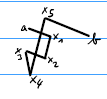
\includegraphics[width=3 cm,height=2cm]{bsp kap 15.11}
	\end{figure}\\ 
	Man nennt eibe solche Folge $a,x_1,x_2,...,x_{m-1},b$ oder auch 
	$\overline{ax_1}\cup \overline{x_1x_2}\cup...\cup \overline{x_{m-1}b}$ 
	einen \redul{Streckenzug} oder \redul{Polygonzug}.\\
	\\
	\textbf{15.12. \underline{Satz:}} \underline{Vor.:} $M\subset 
	\mathbb{R}^n.$ \underline{Beh.:} M \greenul{Gebiet} $\Leftrightarrow$ M 
	\greenul{polygonzush.} $\Leftrightarrow$ M \greenul{wegzush.}\\
	\underline{Bew.}(durch Ringschluss):\\
	(i) \underline{Z.z.:} \oraul{M Gebiet $\Leftrightarrow$ M polygonzush.}:\\
	Sei $x\in M$ bel. Setze \yelul{V=}$V_x:=\{b \in M; b\text{mit x 
	\oraul{durch Polygonzug verbindbar}}\}$\\
	$=\{b \in M; \exists x_1,...,x_k \in M: 
	\overline{bx_1}\cup\overline{x_1x_2}\cup...\cup \overline{x_kx} \subseteq 
	M\}$.\\
	Da $ a \in V$, ist $V\neq \o$.\\
	$\bullet$ Haben: \oraul{V ist offen}, d.h. $b \in V 
	\overset{!}{\Leftrightarrow} \exists B_b^\epsilon \subseteq V.\\$
	\textopencorner Denn: M offen $\Rightarrow\exists \epsilon \textgreater 0: 
	B_b^\epsilon \subseteq M$.\\
	Sei $c \in B_b^\epsilon.$ Wegen $\overline{bc}\subseteq B_b^\epsilon$ folgt 
	dann $c\in V,$ d.h. $B_b^\epsilon\subseteq V$.\textcorner\\
	$\bullet$ Haben: \oraul{V ist abg.}, d.h. $CV$ ist offen.\\
	Dazu betr. $B_b^\epsilon M$ für $b\in \dot{V}.\\$
	Haben $B_b^\epsilon \backslash \{b\}\cap V \neq \o$, wähle $c \in V\cap 
	B_b^\epsilon, c\neq b\\
	\Rightarrow \overline{vc} \subseteq B_b^\epsilon \Rightarrow b \in V$. Es 
	folgt $\overline{V}=V\cup\dot{V}\subseteq V$, also $\overline{V}=V$, d.h. 
	ist abg.\\
	(ii): \oraul{M polygonzush. $\Rightarrow$ M wegzush.}: trivial, da 
	Streckenzüge Wege sind.\\
	(iii): \oraul{M wegzush. $\Rightarrow$ M Gebiet}:\\
	\underline{Zeige:} \oraul{M zush. $\Leftarrow \forall x,y \in M \exists Z 
	\subseteq\textcolor{blue}{M}$:$x,y\in Z,Z$ zush.}\\
	\textopencorner Sei $f:M\rightarrow \mathbb{Z}$ stetig, $y\in M$. Ist $x 
	\in M$ bel., so gibt es ein $Z\subseteq M, Z$ zush., $x,y\in Z$, nach Vor.\\
	Betr. $f_{rZ}$. Diese Abb. ist stetig, und da Z zush. ist, ist $f_{rZ}$ 
	Konstant nach \blueul{Hilfssatz $\blackcircle{*}$ 15.6."$\Rightarrow$"}.\\
	Es folgt f(x)=f(y). Da $x,y\in M$ bel., ist f auf M konstant.\\
	Mit \blueul{Hilfssatz $\blackcircle{*}$ 15.6. "$\Rightarrow$"}, folgt: M 
	zush.\textcorner\\
	\\
	Mit dieser Beh. folgt (iii), denn von x nach y führt eien Weg in M um jeden 
	Punkt des Weges wähle eine $\epsilon$-Umg. ganz in M. Setze Z als 
	Vereinigung aller dieser $\epsilon$-Umg.\\
	\\
	\redcircle{Ü} Eine Vereinigung nicht disjunkter zush. Mengen ist zush.\\
	\\
	\textbf{15.13. \underline{Kor.:}} $\o \neq M \subseteq \mathbb{R}^1: M$ 
	\greenul{zush.} $\Leftrightarrow$ M \greenul{Intervall}.\\
	\textopencorner denn \oraul{IVe in $\mathbb{R}^1$} sind per Def. 
	\oraul{wegzusammenhängend}\textcorner\\
	\\
	\textbf{15.14. \underline{Kor.:}} f:\greenul{$R\rightarrow\mathbb{R}^1$ 
	stetig, R zush.} $\overset{\text{\blueul{15.6.}}}{\Rightarrow}$ 
	\greenul{f(R) zush.} 
	$\overset{\text{\blueul{15.4.}}}{\Rightarrow}$\greenul{f(R) 
	Intervall}.\\
	Dies ist wieder der \blueul{Satz von Min./Max. An9.30.}, es folgt der 
	\blueul{ZWS An9.29.}\\
	\\
	\textbf{15.15. \underline{Bem.:}} Die Relation \redul{x~y}: 
	$\Leftrightarrow \exists Z \subseteq M, Z$ zush.: $x,y\in Z$\\
	ist auf $M \subseteq R$ (R ein metrischer Raum) eine 
	\greenul{Äquivalenzrelation} \textopencorner reflexiv $\checkmark$ 
	symmetrisch $\checkmark$ transitiv$\checkmark$\textcorner auf M.\\
	Haben auch \greenul{x~y $\Leftrightarrow x\in V_y \Leftrightarrow y \in 
	V_x$} laut Beweis von \blueul{15.12.} in $R=\mathbb{R}^n$.\\
	Die Äquivalenzklassen sind \greenul{zush. und abg.} Da M disjunkte 
	Vereinigung dieser Ä-Klassen ist, heißen duese due 
	\redul{Zusammenhangskomponenten von M}. Schränkt man eine stetige Fkt. 
	$f:M\rightarrow \mathbb{Z}$ ein auf eine \greenul{Zush. Komponente U},\\
	so ist \greenul{$f_{rU}$ Konstant} laut \blueul{15.6.}, und die 
	\greenul{Urbilder einpunktiger Mengen $\{a\}\subseteq \mathbb{Z}$} sind 
	\greenul{Vereinigungen von Zusammenhangskomponenten von M}.
\end{document}